\documentclass[letterpaper,titlepage]{article}
\usepackage[margin=1in,dvips]{geometry}
\usepackage{graphicx,float,psfrag,amsmath,amsthm,amssymb}
\usepackage{natbib}
\usepackage{url,color,booktabs}
\usepackage{hyperref}
% Miguel A. Carreira-Perpinan's LaTeX macros.
% Time-stamp: <17/07/10 15:04:36 mcarreira-perpinan>

% Definitions that require only standard LaTeX2e things

% Test whether an argument is empty: []
\def \ifempty#1{\def\temp{#1} \ifx\temp\empty }


% Letters used for matrices and vectors (boldface), for functions (roman), etc.
\newcommand{\A}{\ensuremath{\mathbf{A}}}
\newcommand{\B}{\ensuremath{\mathbf{B}}}
\newcommand{\C}{\ensuremath{\mathbf{C}}}
\newcommand{\D}{\ensuremath{\mathbf{D}}}
\newcommand{\E}{\ensuremath{\mathbf{E}}}
\newcommand{\F}{\ensuremath{\mathbf{F}}}
\newcommand{\G}{\ensuremath{\mathbf{G}}}
\newcommand{\HH}{\ensuremath{\mathbf{H}}}
\newcommand{\I}{\ensuremath{\mathbf{I}}}
\newcommand{\J}{\ensuremath{\mathbf{J}}}
\newcommand{\K}{\ensuremath{\mathbf{K}}}
\newcommand{\LL}{\ensuremath{\mathbf{L}}}
\newcommand{\M}{\ensuremath{\mathbf{M}}}
\newcommand{\N}{\ensuremath{\mathbf{N}}}
\newcommand{\OO}{\ensuremath{\mathbf{O}}}
\newcommand{\PP}{\ensuremath{\mathbf{P}}}
\newcommand{\Q}{\ensuremath{\mathbf{Q}}}
%\newcommand{\R}{\ensuremath{\mathbf{R}}} % PROSPER defines \R
\newcommand{\RR}{\ensuremath{\mathbf{R}}}
\renewcommand{\SS}{\ensuremath{\mathbf{S}}}
\newcommand{\T}{\ensuremath{\mathbf{T}}}
\newcommand{\U}{\ensuremath{\mathbf{U}}}
\newcommand{\V}{\ensuremath{\mathbf{V}}}
\newcommand{\W}{\ensuremath{\mathbf{W}}}
\newcommand{\X}{\ensuremath{\mathbf{X}}}
\newcommand{\Y}{\ensuremath{\mathbf{Y}}}
\newcommand{\Z}{\ensuremath{\mathbf{Z}}}
\renewcommand{\aa}{\ensuremath{\mathbf{a}}}
\renewcommand{\b}{\ensuremath{\mathbf{b}}}
\renewcommand{\c}{\ensuremath{\mathbf{c}}}
\newcommand{\dd}{\ensuremath{\mathbf{d}}}
\newcommand{\e}{\ensuremath{\mathbf{e}}}
\newcommand{\f}{\ensuremath{\mathbf{f}}}
\newcommand{\g}{\ensuremath{\mathbf{g}}}
\newcommand{\h}{\ensuremath{\mathbf{h}}}
\newcommand{\bk}{\ensuremath{\mathbf{k}}}
\newcommand{\bl}{\ensuremath{\mathbf{l}}}
\newcommand{\m}{\ensuremath{\mathbf{m}}}
\newcommand{\n}{\ensuremath{\mathbf{n}}}
\newcommand{\p}{\ensuremath{\mathbf{p}}}
\newcommand{\q}{\ensuremath{\mathbf{q}}}
\newcommand{\rr}{\ensuremath{\mathbf{r}}}
\newcommand{\sss}{\ensuremath{\mathbf{s}}}  % TIPA defines \s and LaTeX \ss!
\renewcommand{\t}{\ensuremath{\mathbf{t}}}
\newcommand{\uu}{\ensuremath{\mathbf{u}}}
\newcommand{\vv}{\ensuremath{\mathbf{v}}}
%\renewcommand{\v}{\ensuremath{\mathbf{v}}}
\newcommand{\w}{\ensuremath{\mathbf{w}}}
\newcommand{\x}{\ensuremath{\mathbf{x}}}
\newcommand{\y}{\ensuremath{\mathbf{y}}}
\newcommand{\z}{\ensuremath{\mathbf{z}}}
\newcommand{\0}{\ensuremath{\mathbf{0}}}
\newcommand{\1}{\ensuremath{\mathbf{1}}}

% Bold symbols and greek letters
\newcommand{\balpha}{\ensuremath{\boldsymbol{\alpha}}}
\newcommand{\bbeta}{\ensuremath{\boldsymbol{\beta}}}
\newcommand{\bdelta}{\ensuremath{\boldsymbol{\delta}}}
\newcommand{\bepsilon}{\ensuremath{\boldsymbol{\epsilon}}}
\newcommand{\bgamma}{\ensuremath{\boldsymbol{\gamma}}}
\newcommand{\binfty}{\ensuremath{\boldsymbol{\infty}}}
\newcommand{\bkappa}{\ensuremath{\boldsymbol{\kappa}}}
\newcommand{\blambda}{\ensuremath{\boldsymbol{\lambda}}}
\newcommand{\bmu}{\ensuremath{\boldsymbol{\mu}}}
\newcommand{\bnu}{\ensuremath{\boldsymbol{\nu}}}
\newcommand{\bphi}{\ensuremath{\boldsymbol{\phi}}}
\newcommand{\bpi}{\ensuremath{\boldsymbol{\pi}}}
\newcommand{\bpsi}{\ensuremath{\boldsymbol{\psi}}}
\newcommand{\brho}{\ensuremath{\boldsymbol{\rho}}}
\newcommand{\bsigma}{\ensuremath{\boldsymbol{\sigma}}}
\newcommand{\btau}{\ensuremath{\boldsymbol{\tau}}}
\newcommand{\btheta}{\ensuremath{\boldsymbol{\theta}}}
\newcommand{\bxi}{\ensuremath{\boldsymbol{\xi}}}
\newcommand{\bzeta}{\ensuremath{\boldsymbol{\zeta}}}

\newcommand{\bDelta}{\ensuremath{\boldsymbol{\Delta}}}
\newcommand{\bGamma}{\ensuremath{\boldsymbol{\Gamma}}}
\newcommand{\bLambda}{\ensuremath{\boldsymbol{\Lambda}}}
\newcommand{\bPhi}{\ensuremath{\boldsymbol{\Phi}}}
\newcommand{\bPi}{\ensuremath{\boldsymbol{\Pi}}}
\newcommand{\bPsi}{\ensuremath{\boldsymbol{\Psi}}}
\newcommand{\bSigma}{\ensuremath{\boldsymbol{\Sigma}}}
\newcommand{\bTheta}{\ensuremath{\boldsymbol{\Theta}}}
\newcommand{\bXi}{\ensuremath{\boldsymbol{\Xi}}}
\newcommand{\bUpsilon}{\ensuremath{\boldsymbol{\Upsilon}}}

% Blackboard bold
\newcommand{\bbC}{\ensuremath{\mathbb{C}}}
\newcommand{\bbH}{\ensuremath{\mathbb{H}}}
\newcommand{\bbN}{\ensuremath{\mathbb{N}}}
\newcommand{\bbR}{\ensuremath{\mathbb{R}}}
\newcommand{\bbS}{\ensuremath{\mathbb{S}}}
\newcommand{\bbZ}{\ensuremath{\mathbb{Z}}}
\newcommand{\bbE}{\ensuremath{\mathbb{E}}}
\newcommand{\bbT}{\ensuremath{\mathbb{T}}}


% Calligraphic
\newcommand{\calA}{\ensuremath{\mathcal{A}}}
\newcommand{\calB}{\ensuremath{\mathcal{B}}}
\newcommand{\calC}{\ensuremath{\mathcal{C}}}
\newcommand{\calD}{\ensuremath{\mathcal{D}}}
\newcommand{\calE}{\ensuremath{\mathcal{E}}}
\newcommand{\calF}{\ensuremath{\mathcal{F}}}
\newcommand{\calG}{\ensuremath{\mathcal{G}}}
\newcommand{\calH}{\ensuremath{\mathcal{H}}}
\newcommand{\calI}{\ensuremath{\mathcal{I}}}
\newcommand{\calJ}{\ensuremath{\mathcal{J}}}
\newcommand{\calK}{\ensuremath{\mathcal{K}}}
\newcommand{\calL}{\ensuremath{\mathcal{L}}}
\newcommand{\calM}{\ensuremath{\mathcal{M}}}
\newcommand{\calN}{\ensuremath{\mathcal{N}}}
\newcommand{\calO}{\ensuremath{\mathcal{O}}}
\newcommand{\calP}{\ensuremath{\mathcal{P}}}
\newcommand{\calR}{\ensuremath{\mathcal{R}}}
\newcommand{\calS}{\ensuremath{\mathcal{S}}}
\newcommand{\calT}{\ensuremath{\mathcal{T}}}
\newcommand{\calU}{\ensuremath{\mathcal{U}}}
\newcommand{\calV}{\ensuremath{\mathcal{V}}}
\newcommand{\calW}{\ensuremath{\mathcal{W}}}
\newcommand{\calX}{\ensuremath{\mathcal{X}}}
\newcommand{\calY}{\ensuremath{\mathcal{Y}}}
\newcommand{\calZ}{\ensuremath{\mathcal{Z}}}

% Relational operators
% \bydef puts ``def'' over the equals sign and means ``is by definition
% equal to''. Another possibility is to use the \triangleq symbol.
\newcommand{\bydef}{\stackrel{\mathrm{\scriptscriptstyle def}}{=}}
% \simbydef puts ``def'' over the ~ sign and means ``is by definition
% distributed as''.
\newcommand{\simbydef}{\stackrel{\mathrm{\scriptscriptstyle def}}{\sim}}
\newcommand{\proptobydef}{\stackrel{\mathrm{\scriptscriptstyle def}}{\propto}}

% Other functions
\newcommand{\ceil}[1]{\lceil#1\rceil}
\newcommand{\floor}[1]{\lfloor#1\rfloor}
% These accept delimiters as arguments: \big \Big \bigg \Bigg.
% Default: \left ... \right.
\newcommand{\abs}[2][]{%
  \ifempty{#1} {\left\lvert#2\right\rvert} \else {#1\lvert#2#1\rvert} \fi}
\newcommand{\norm}[2][]{%
  \ifempty{#1} {\left\lVert#2\right\rVert} \else {#1\lVert#2#1\rVert} \fi}

% Left superscript
% (from http://www.maths.univ-rennes1.fr/~edix/sgahtml/typesetting_rules.html)
\newcommand{\leftexp}[2]{{\vphantom{#2}}^{#1}{#2}}

% Box of text (for pictures, tables, etc.), without frames. Arguments:
%   #1: separation between rows of text as a multiple of LaTeX's default
%       (optional, default 1).
%   #2: position (one of t, b, c).
%   #3: format (one of l, r, c or even p{2cm}).
%   #4: text, which can include line breaks (\\).
\newcommand{\caja}[4][1]{{%
    \renewcommand{\arraystretch}{#1}%
    \begin{tabular}[#2]{@{}#3@{}}%
      #4%
    \end{tabular}%
    }}

% The amsart class has its own \keywords command, in which case we
% don't replace it.
\providecommand{\keywords}[1]{\vspace*{0.5\baselineskip}\par\noindent\textbf{Keywords:} #1}

% The logos (AmSLaTeX, BibTeX, etc.) are defined in texnames.sty.

% List environments
%
% "simplelist": useful for compact lists. Use it instead of "itemize".
% Optional argument: the bullet (default \triangleright). Other nice
% bullets are available in the Zapf Dingbats font (e.g. \ding{166} in
% the pifont package).
%
\newenvironment{simplelist}[1][$\triangleright$]%
{%
\begin{list}{#1}{
\vspace{-\topsep}
\vspace{-\partopsep}
\setlength{\itemindent}{0cm}
\setlength{\rightmargin}{0cm}
\setlength{\listparindent}{0cm}
\settowidth{\labelwidth}{#1}
\setlength{\leftmargin}{\labelwidth}
\addtolength{\leftmargin}{\labelsep}
\setlength{\itemsep}{0cm}
%\setlength{\leftmargin}{0cm}
%\setlength{\labelwidth}{0cm}
}%
}%
{%
\end{list}
\vspace{-\topsep}
\vspace{-\partopsep}
}

%
% enumthm: an enumerated list intended to appear in theorems and not
% to be nested. Each item is numbered in Roman numerals in parentheses.
% A suitable way to refer to an item is:
% Theorem~\ref{thm:pithagoras}(\ref{en:triangle}) states...
\newenvironment{enumthm}%
{\begin{enumerate}%
\renewcommand{\theenumi}{\roman{enumi}}%
\renewcommand{\labelenumi}{(\theenumi)}}%
{\end{enumerate}}

% Commands for the hyperref package (they also require the url package).
% In all cases the typesetting style is tt by default but can be changed
% with the \urlstyle command, e.g. \urlstyle{tt}.
%
% \MACPhref[text]{link} typesets text (default = link) in tt and
% hyperlinks to link, e.g. \MACPhref{http://www.dcs.shef.ac.uk/~miguel}.
\newcommand{\MACPhref}[2][\DefaultOpt]{\def\DefaultOpt{#2}%
  \href{#2}{\url{#1}}}
%
% \MACPmailto[text]{email} typesets text (default = email) in tt and
% hyperlinks to email as mailto:email, e.g. \MACPmailto{miguel@dcs.shef.ac.uk}.
\newcommand{\MACPmailto}[2][\DefaultOpt]{\def\DefaultOpt{#2}%
  \href{mailto:#2}{\url{#1}}}

% % Hyphenation
% \hyphenation{elec-tro-pa-la-tog-ra-phy}

% % From the amsbook.cls file version 2.04
% \hyphenation{acad-e-my acad-e-mies af-ter-thought anom-aly anom-alies
% an-ti-deriv-a-tive an-tin-o-my an-tin-o-mies apoth-e-o-ses
% apoth-e-o-sis ap-pen-dix ar-che-typ-al as-sign-a-ble as-sist-ant-ship
% as-ymp-tot-ic asyn-chro-nous at-trib-uted at-trib-ut-able bank-rupt
% bank-rupt-cy bi-dif-fer-en-tial blue-print busier busiest
% cat-a-stroph-ic cat-a-stroph-i-cally con-gress cross-hatched data-base
% de-fin-i-tive de-riv-a-tive dis-trib-ute dri-ver dri-vers eco-nom-ics
% econ-o-mist elit-ist equi-vari-ant ex-quis-ite ex-tra-or-di-nary
% flow-chart for-mi-da-ble forth-right friv-o-lous ge-o-des-ic
% ge-o-det-ic geo-met-ric griev-ance griev-ous griev-ous-ly
% hexa-dec-i-mal ho-lo-no-my ho-mo-thetic ideals idio-syn-crasy
% in-fin-ite-ly in-fin-i-tes-i-mal ir-rev-o-ca-ble key-stroke
% lam-en-ta-ble light-weight mal-a-prop-ism man-u-script mar-gin-al
% meta-bol-ic me-tab-o-lism meta-lan-guage me-trop-o-lis
% met-ro-pol-i-tan mi-nut-est mol-e-cule mono-chrome mono-pole
% mo-nop-oly mono-spline mo-not-o-nous mul-ti-fac-eted mul-ti-plic-able
% non-euclid-ean non-iso-mor-phic non-smooth par-a-digm par-a-bol-ic
% pa-rab-o-loid pa-ram-e-trize para-mount pen-ta-gon phe-nom-e-non
% post-script pre-am-ble pro-ce-dur-al pro-hib-i-tive pro-hib-i-tive-ly
% pseu-do-dif-fer-en-tial pseu-do-fi-nite pseu-do-nym qua-drat-ic
% quad-ra-ture qua-si-smooth qua-si-sta-tion-ary qua-si-tri-an-gu-lar
% quin-tes-sence quin-tes-sen-tial re-arrange-ment rec-tan-gle
% ret-ri-bu-tion retro-fit retro-fit-ted right-eous right-eous-ness
% ro-bot ro-bot-ics sched-ul-ing se-mes-ter semi-def-i-nite
% semi-ho-mo-thet-ic set-up se-vere-ly side-step sov-er-eign spe-cious
% spher-oid spher-oid-al star-tling star-tling-ly sta-tis-tics
% sto-chas-tic straight-est strange-ness strat-a-gem strong-hold
% sum-ma-ble symp-to-matic syn-chro-nous topo-graph-i-cal tra-vers-a-ble
% tra-ver-sal tra-ver-sals treach-ery turn-around un-at-tached
% un-err-ing-ly white-space wide-spread wing-spread wretch-ed
% wretch-ed-ly Eng-lish Euler-ian Feb-ru-ary Gauss-ian
% Hamil-ton-ian Her-mit-ian Jan-u-ary Japan-ese Kor-te-weg
% Le-gendre Mar-kov-ian Noe-ther-ian No-vem-ber Rie-mann-ian Sep-tem-ber}

%%% Local Variables: 
%%% mode: latex
%%% TeX-master: t
%%% End: 

% Definitions that require the amsmath.sty and amsthm.sty files
% Time-stamp: <16/02/05 18:07:53 mcarreira-perpinan>

% -------------- Operators --------------

\DeclareMathOperator*{\argmin}{arg\,min}
\DeclareMathOperator*{\argmax}{arg\,max}

% Probability
\newcommand{\Eop}{\operatorname{E}}
\newcommand{\mean}[2][]{\ensuremath{\Eop_{#1}\left\{#2\right\}}}
\newcommand{\meanop}{\operatorname{mean}}
\newcommand{\Mean}[2][]{\ensuremath{\meanop_{#1}\left\{#2\right\}}}
\newcommand{\aveop}{\Eop}
\newcommand{\ave}[2][]{\ensuremath{\aveop_{#1}\left\{#2\right\}}}
\newcommand{\varop}{\operatorname{var}}
\newcommand{\var}[2][]{\ensuremath{\varop_{#1}\left\{#2\right\}}}
\newcommand{\stdevop}{\operatorname{stdev}}
\newcommand{\stdev}[2][]{\ensuremath{\stdevop_{#1}\left\{#2\right\}}}
\newcommand{\covop}{\operatorname{cov}}
\newcommand{\cov}[2][]{\ensuremath{\covop_{#1}\left\{#2\right\}}}
\newcommand{\eff}{\operatorname{eff}}
\newcommand{\Prop}{\operatorname{Pr}}
\newcommand{\prob}[1]{\ensuremath{\Prop\left[#1\right]}}
\newcommand{\Volume}{\operatorname{vol}}
\newcommand{\volume}[1]{\ensuremath{\Volume\left(#1\right)}}
\newcommand{\Domain}{\operatorname{dom}}
\newcommand{\dom}[1]{\ensuremath{\Domain\left(#1\right)}}

% Functions
\newcommand{\erf}{\operatorname{erf}}
\newcommand{\sgnop}{\operatorname{sgn}}
\newcommand{\sgn}[1]{\ensuremath{\sgnop\left(#1\right)}}

% Information theory
\newcommand{\KLop}{\operatorname{D}}
%\newcommand{\KLop}{\operatorname{KL}}
\newcommand{\KL}[2]{\KLop\left(#1\lVert#2\right)} % Kullback-Leibler divergence
\newcommand{\KLsym}[2]{\KLop\left(#1,#2\right)}   % Symmetrised KL divergence

% Set theory
% Are "card" and "im" the correct names in English?
\newcommand{\cardop}{\operatorname{card}}
\newcommand{\card}[1]{\ensuremath{\cardop\left(#1\right)}}
\newcommand{\im}{\operatorname{im}}
\newcommand{\vol}{\operatorname{vol}}
\newcommand{\convop}{\operatorname{conv}}
\newcommand{\conv}[1]{\ensuremath{\convop\left(#1\right)}}

% Matrices
\newcommand{\diagop}{\operatorname{diag}}
\newcommand{\diag}[1]{\ensuremath{\diagop\left(#1\right)}}
\newcommand{\cof}{\operatorname{cof}}           % Cofactor of a matrix element
\newcommand{\adj}{\operatorname{adj}}           % Adjunt matrix
\newcommand{\traceop}{\operatorname{tr}}
\newcommand{\trace}[1]{\ensuremath{\traceop\left(#1\right)}}
\newcommand{\rankop}{\operatorname{rank}}
\newcommand{\rank}[1]{\ensuremath{\rankop\left(#1\right)}}
\newcommand{\Nullop}{\operatorname{null}}
\newcommand{\Null}[1]{\ensuremath{\Nullop\left(#1\right)}}
\newcommand{\rangeop}{\operatorname{range}}
\newcommand{\range}[1]{\ensuremath{\rangeop\left(#1\right)}}
\newcommand{\Dimop}{\operatorname{dim}}
\newcommand{\Dim}[1]{\ensuremath{\Dimop\left(#1\right)}}
\newcommand{\spanop}{\operatorname{span}}
\newcommand{\spn}[1]{\ensuremath{\spanop\left\{#1\right\}}}
\newcommand{\vectop}{\operatorname{vec}}
\newcommand{\vect}[1]{\ensuremath{\vectop\left(#1\right)}}
\newcommand{\condop}{\operatorname{cond}}
\newcommand{\cond}[1]{\ensuremath{\condop\left(#1\right)}}

% Other
\newcommand{\proxop}{\operatorname{prox}}
\newcommand{\prox}[2]{\ensuremath{\proxop_{#1}\left(#2\right)}}


% Definitions that require the amsmath.sty and amsthm.sty files
% Time-stamp: <16/02/05 18:08:09 mcarreira-perpinan>

% -------------- Theorem environments --------------
\theoremstyle{plain}% default
\newtheorem{thm}{Theorem}[section]
\newtheorem{lemma}[thm]{Lemma}
\newtheorem*{lemma*}{Lemma}
\newtheorem{prop}[thm]{Proposition}
\newtheorem*{prop*}{Proposition}
\newtheorem{cor}[thm]{Corollary}
\newtheorem{obs}[thm]{Observation}
\newtheorem{ass}[thm]{Assumption}

\theoremstyle{definition}
\newtheorem{defn}{Definition}[section]
\newtheorem*{defn*}{Definition}
\newtheorem{exmp}{Example}[section]
\newtheorem*{exmp*}{Example}
\newtheorem{conj}{Conjecture}[section]
\newtheorem*{conj*}{Conjecture}

\theoremstyle{remark}
\newtheorem{rmk}[thm]{Remark}
\newtheorem*{rmk*}{Remark}



\graphicspath{{grf/},{plot/}}

\bibpunct[, ]{(}{)}{;}{a}{,}{,} % Should be the natbib 
\begin{document}

\section{Experiments and Applications}

\subsection{Toy Task: The Rooms Problem}
To provide an illustration of HRL in action, we apply the subgoal discovery algorithm to the \emph{Rooms problem} introduced by \citep{RL-Book:Sutton:1998}. Given initial state $S$ and goal state $G$, the agent's task is to navigate through a set of rooms interconnected by doorways, in order to reach the goal state $G$ (Figure \ref{g:4-room}). In each state, the agent can select any of eight deterministic primitive actions, each of which moves the agent to one of the adjacent squares (unless a wall prevents this movement). The rooms are reachable through \emph{doors} and agent is only allowed to use these doors to reach the other room. Agent receives reward of $-1$ for each action, $-2$ for actions that results bumping to the walls and $0$ when reaching to $G$. 
\begin{figure}[H]
\centering
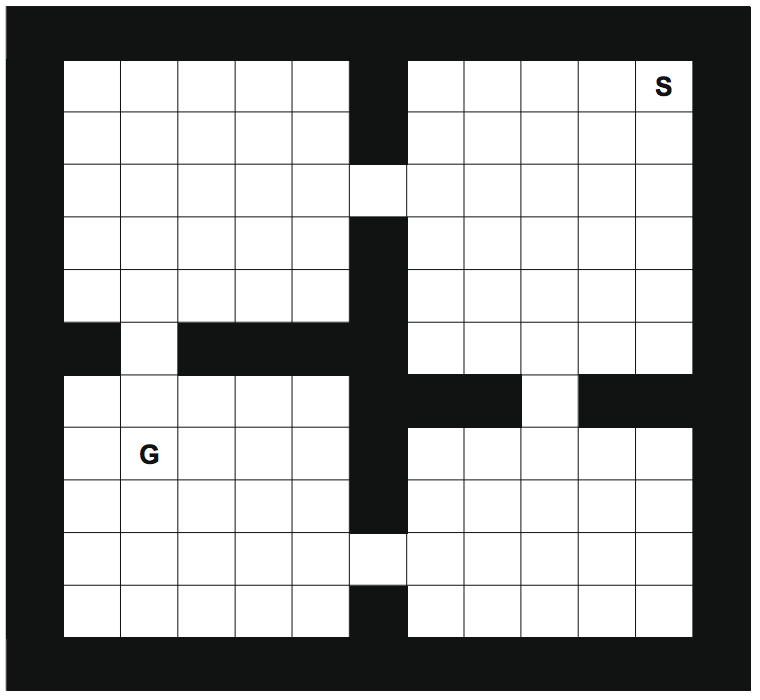
\includegraphics[width=0.5\textwidth]{4-room.png}
\caption{The rooms problem, adapted from \citep{HRL-BOTVINICK:2009}}
\label{g:4-room}
\end{figure}

\subsection{ATARI Games: Montezuma's Revenge}
The Arcade Learning Environment (ALE) is an evaluation platform that provides an interface to hundreds of Atari 2600 game environments. It supports a variety of different problem settings and it has been receiving increasing attention from the scientific community, leading to some high-profile success stories such as the much publicized Deep Q-Networks (DQN) \citep{DeepMind-ATARI-2013,ALE:Bellemare:2013}. Montezuma's revenge is one of the hardest games available through ALE. The game is infamous for challenging agents with lethal traps and sparse rewards \citep{FeUdal:HRL:Sahsa:2017}. The game (Figure \ref{g:montezuma-revenge}) requires the player to navigate the explorer (in red) through several rooms while collecting treasures. In order to pass through doors (in the top right and top left corners of the figure), the player has to first pick up the key \citep{HRL:MIT:Kulkarni:2016}. The hierarchical nature of this game made it a common experiment for testing hierarchical reinforcement learning algorithm \citep{HRL:MIT:Kulkarni:2016,FeUdal:HRL:Sahsa:2017}.
\begin{figure}[H]
\centering
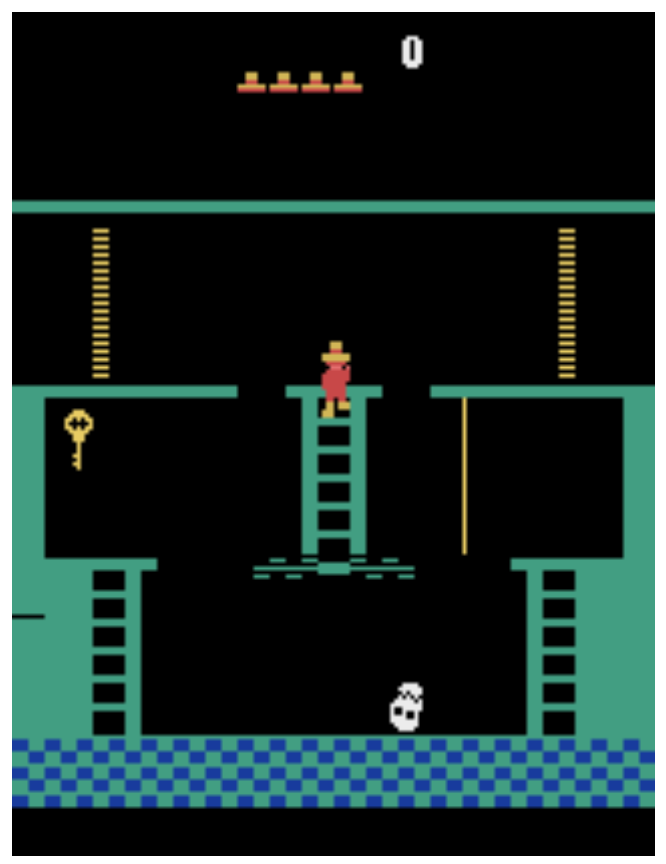
\includegraphics[width=0.5\textwidth]{montezuma-revenge.png}
\caption{A sample screen from the ATARI 2600 game called `'Montezuma's Revenge'' adopted from \citep{HRL:MIT:Kulkarni:2016}}
\label{g:montezuma-revenge}
\end{figure}

\subsection{Path Planning for Autonoumous Robot Navigation}
Navigation is one of the most important robotic tasks. One classic approach consists of three steps: build a map of the environment through, e.g., Simultaneous Localization and Mapping (SLAM), plan a path using the map, and finally execute the path. High-fidelity geometric maps make it easier for path planning and execution. However, building such maps is time-consuming \citep{ROBOT-NAVIGATION-Intention-Net:2017}. Further, even small environmental changes may render them partially invalid. Alternatively, the optical flow approach does not use maps at all and relies on the visual perception of the local environment for navigation. While this avoids the difficulty of building and maintaining accurate geometric maps, it is difficult to achieve effective goal-directed global navigation in complex geometric environments without maps. Our approach uses 2-D floor plans available for indoor environments. We use robotics simulator such as Gebezo and Robot Operating System (ROS) to simulate environments for robotics navigation tasks. 

\subsection{Bipedal Locomotion and Reaching Tasks}
Learning physics-based locomotion skills is a difficult problem. With this simulation we aim to learn a variety of environment-aware locomotion skills with a limited amount of prior knowledge. We investigate the task of reaching and also locomotion using two-level hierarchical control framework. Results are demonstrated on a simulated 3D biped \citep{Deep-LOCO:Peng:2017,bipedal-creatures:Geijtenbeek:2013}.
For animating virtual characters, physics based simulation is used by \citep{bipedal-creatures:Geijtenbeek:2013} (Figure \ref{g:bipedal-creatures}). The subgoal discovery algorithm can be applied to the experience space of locomotion task and learning to reach for these animated creatures in hierarchical reinforcement learning framework.  
\begin{figure}[H]
\centering
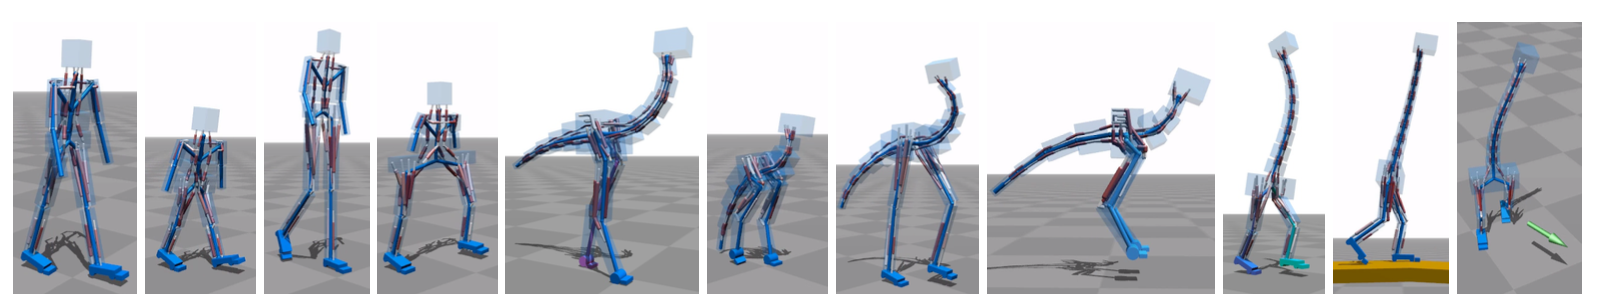
\includegraphics[width=0.9\textwidth]{bipedal-creatures.png}
\caption{Physics-based simulation of locomotion for a variety of creatures driven by 3D muscle-based control adopted from \citep{bipedal-creatures:Geijtenbeek:2013}}
\label{g:bipedal-creatures}
\end{figure}

\subsection{Autonoumous Driving}
The capability of autonomous robotic systems to successfully navigate through difficult environments continues to advance \citep{Autonomous:Silver:2010,Deep-Car-2017,CARLA:2017}.
Driving is usually a navigation task from an initial state to a destination (goal) given the map of the environment. One the most difficult form is navigation in densely populated urban environments due to complex multi-agent dynamics at traffic intersections; the necessity to track and respond to the motion of tens or hundreds of other actors \citep{CARLA:2017}. Training and validation of sensorimotor control models for urban driving in the physical world is beyond the reach of most research groups.
An alternative is to train and validate driving strategies in simulation. There are several open source driving simulators that we will use to test our sub-goal discovery and hierarchical reinforcement learning algorithms in order to approach the complex problem of autonomous driving.

TORCS is a highly portable multi platform car racing simulation. It is used as ordinary car racing game, as AI racing game and as research platform \citep{TORCS} (Figure \ref{g:TORCS}).
\begin{figure}[H]
\centering
\includegraphics[width=0.4\textwidth]{TORCS-2.png}
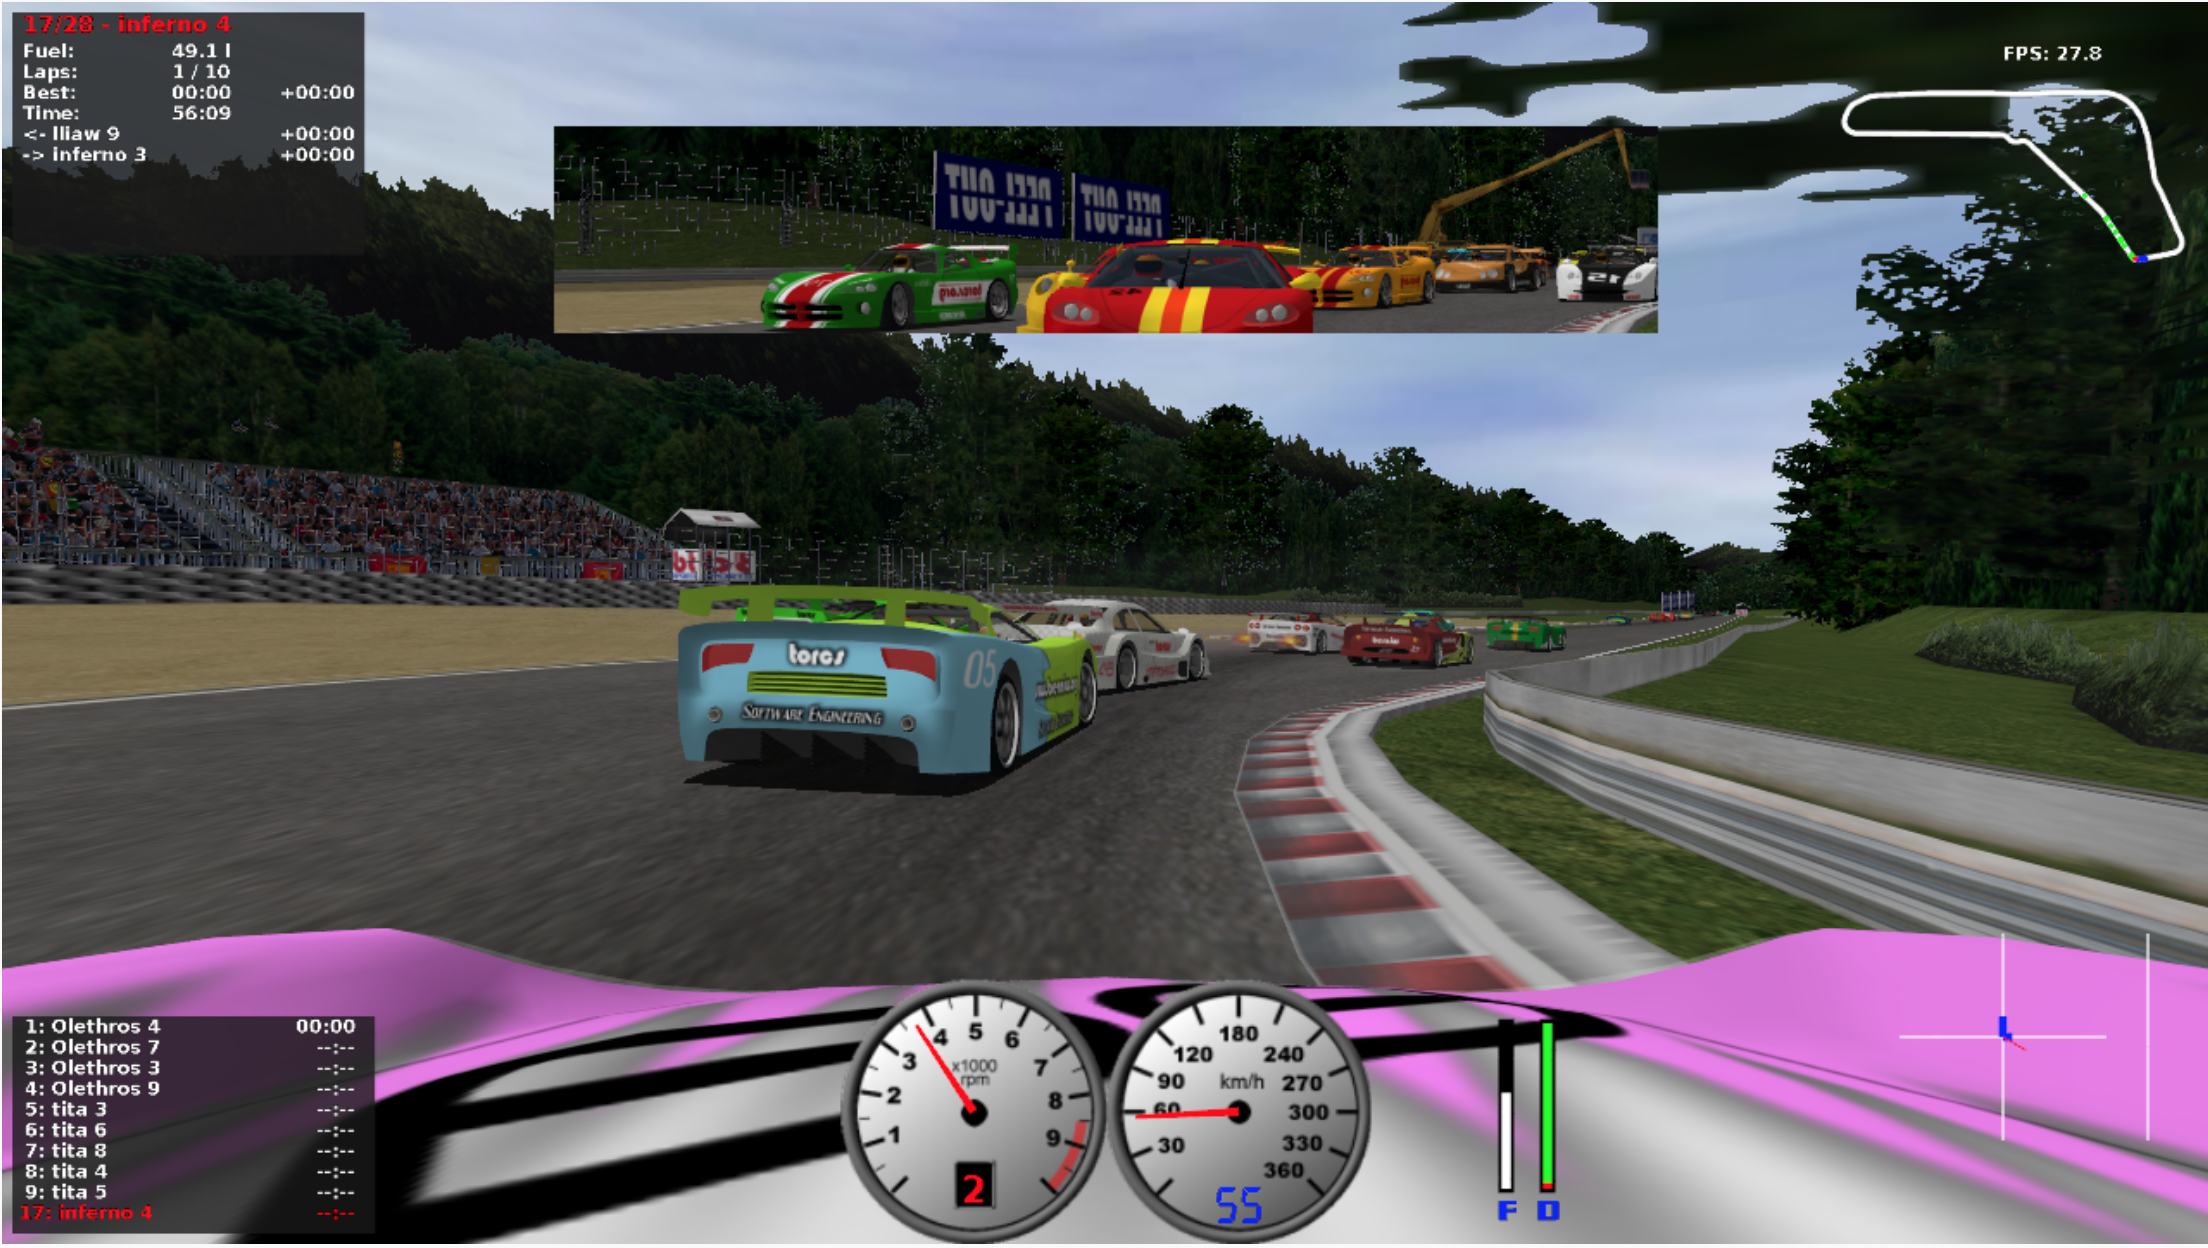
\includegraphics[width=0.4\textwidth]{TORCS-1.png}
\caption{Example shots from \citep{TORCS}. Left: A third-person view. Right: Perception from the driver's perspective shiled.}
\label{g:TORCS}
\end{figure}


CARLA is another open-source simulator for autonomous driving research \citep{CARLA:2017}. CARLA has been built for flexibility and realism in the rendering and physics simulation. It is implemented as an open-source layer over Unreal Engine 4 (UE4). CARLA has been developed from the ground up to support development, training, and validation of autonomous urban driving systems. The simulation platform supports flexible specification of sensor suites and environmental conditions. We use CARLA to study the performance of subgoal discovery algorithms for hierarchical reinforcement learning applied to autonomous driving. We use CARLA to stage controlled goal-directed navigation scenarios of increasing difficulty. We manipulate the complexity of the route that must be traversed, the presence of traffic, and the environmental conditions (Figures \ref{g:CARLA} and \ref{g:CARLA-2}). 
\begin{figure}[H]
\centering
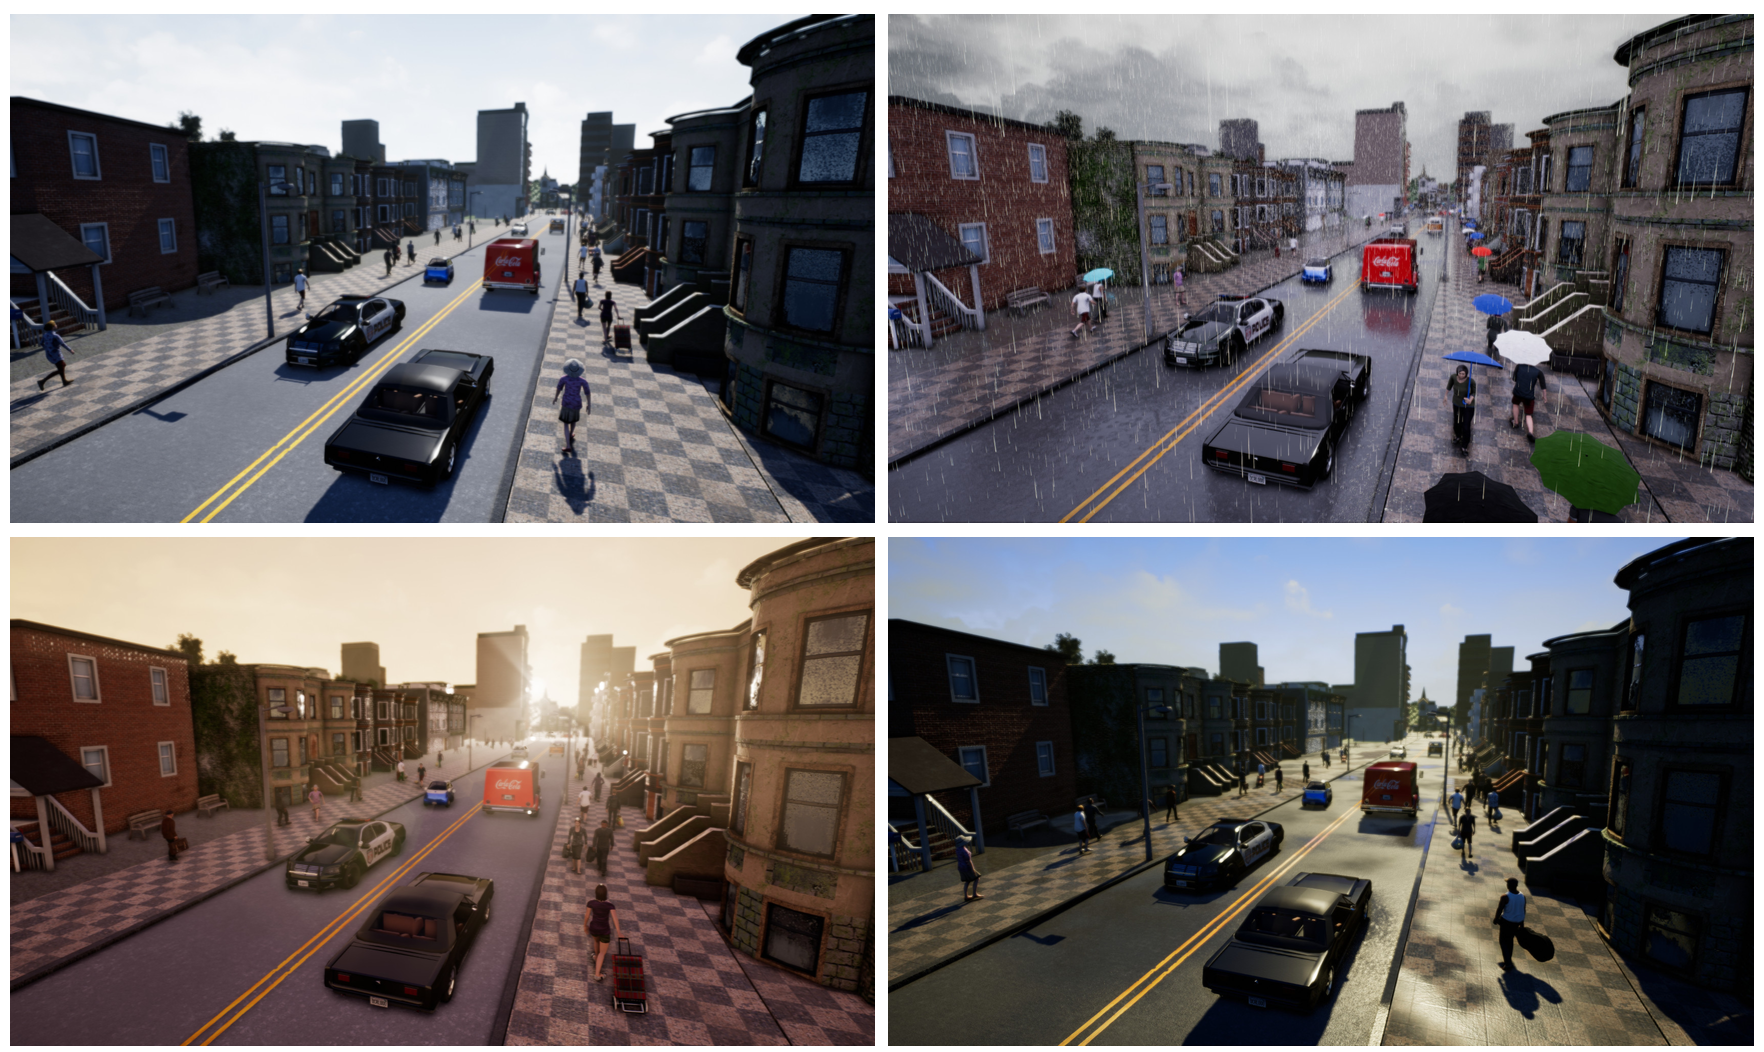
\includegraphics[width=0.8\textwidth]{CARLA.png}
\caption{A third-person view in four weather conditions. Clock- wise from top left: clear day, daytime rain, daytime shortly after rain, and clear sunset adopted from \citep{CARLA:2017}}
\label{g:CARLA}
\end{figure}

\begin{figure}[H]
\centering
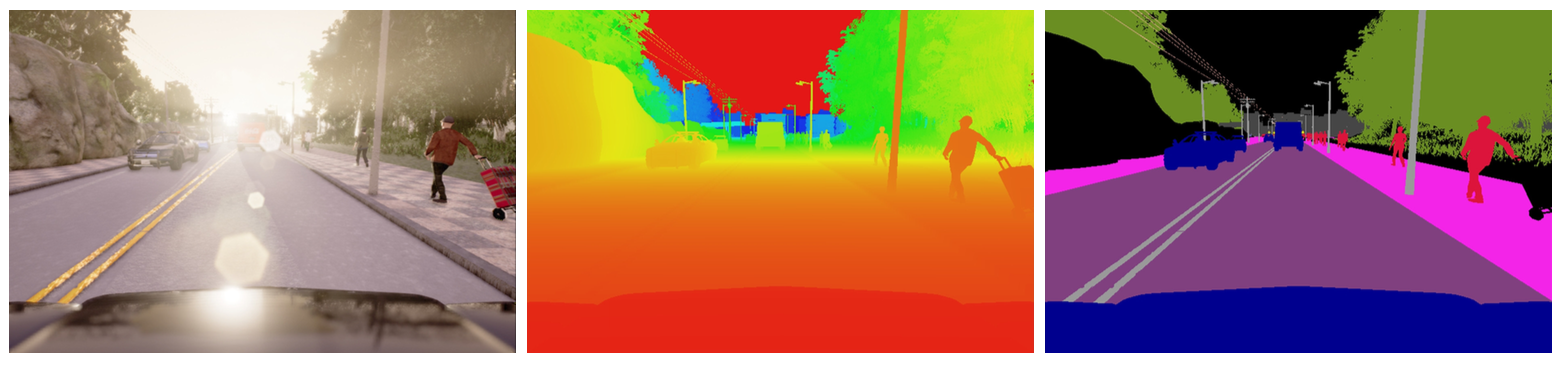
\includegraphics[width=0.8\textwidth]{CARLA-2.png}
\caption{Three of the sensing modalities provided by CARLA. From left to right: normal vision camera, ground-truth depth, and ground-truth semantic segmentation. Depth and semantic segmen- tation are pseudo-sensors that support experiments that control for the role of perception. Additional sensor models can be plugged in via the API adopted from \citep{CARLA:2017}}
\label{g:CARLA-2}
\end{figure}

\newpage
\bibliography{myBib}
\bibliographystyle{apalike}
\end{document}